\documentclass[18pt]{beamer}
\usepackage[utf8]{inputenc}
\usepackage{templates/mytemplate}
\usepackage{templates/beamerthemekit}
\usepackage{graphicx}
\usepackage{microtype}
\usepackage{listings}
\usepackage{color}
\usepackage{hyperref}
\usepackage{multicol}
\usepackage{siunitx}
\usepackage{physics}
\usepackage{appendixnumberbeamer}

\title{Look at CDC Wire Hits in GCR}
\subtitle{Hit Efficiencies and Bad Regions}
\author{\underline{Michael Eliachevitch}}
\date{January 19, 2018}
\titleimage{transparent}
\institute{ETP -- KIT}

\begin{document}
\selectlanguage{english}

\begin{frame}
  \titlepage
\end{frame}

\begin{frame}
  \begin{itemize}
  \item Looked at CDC wire hits in GCR August 2017 data
  \item Distribution of number of CDC hits per wire
  \item Distribution of hit to reco track matching efficiency
    \begin{itemize}
    \item If a wire is hit, what is the probability that this hit is used in a reconstructed track?\\
    \item Due to missing beam background, expected to be high, similar to hit efficiency of track finding
    \end{itemize}
  \item Saw dead and noisy regions. Reasons known?
  \end{itemize}
\end{frame}

\begin{frame}
  \frametitle{On GCR August simulated MC}
  \begin{columns}
    \begin{column}{0.5\textwidth}
      \centering
      Total hits per wire
      \includegraphics[width=1.\textwidth]{figures/hit_efficiency_by_wire/total_hits_per_wire_MC.pdf}
    \end{column}
    \begin{column}{0.5\textwidth}
      \centering
      Fraction of hits in a reco track
      \only<1>{\includegraphics[width=1.\textwidth]{figures/hit_efficiency_by_wire/hit_ratio_matched_by_recotrack_MC.pdf}}
      \only<2>{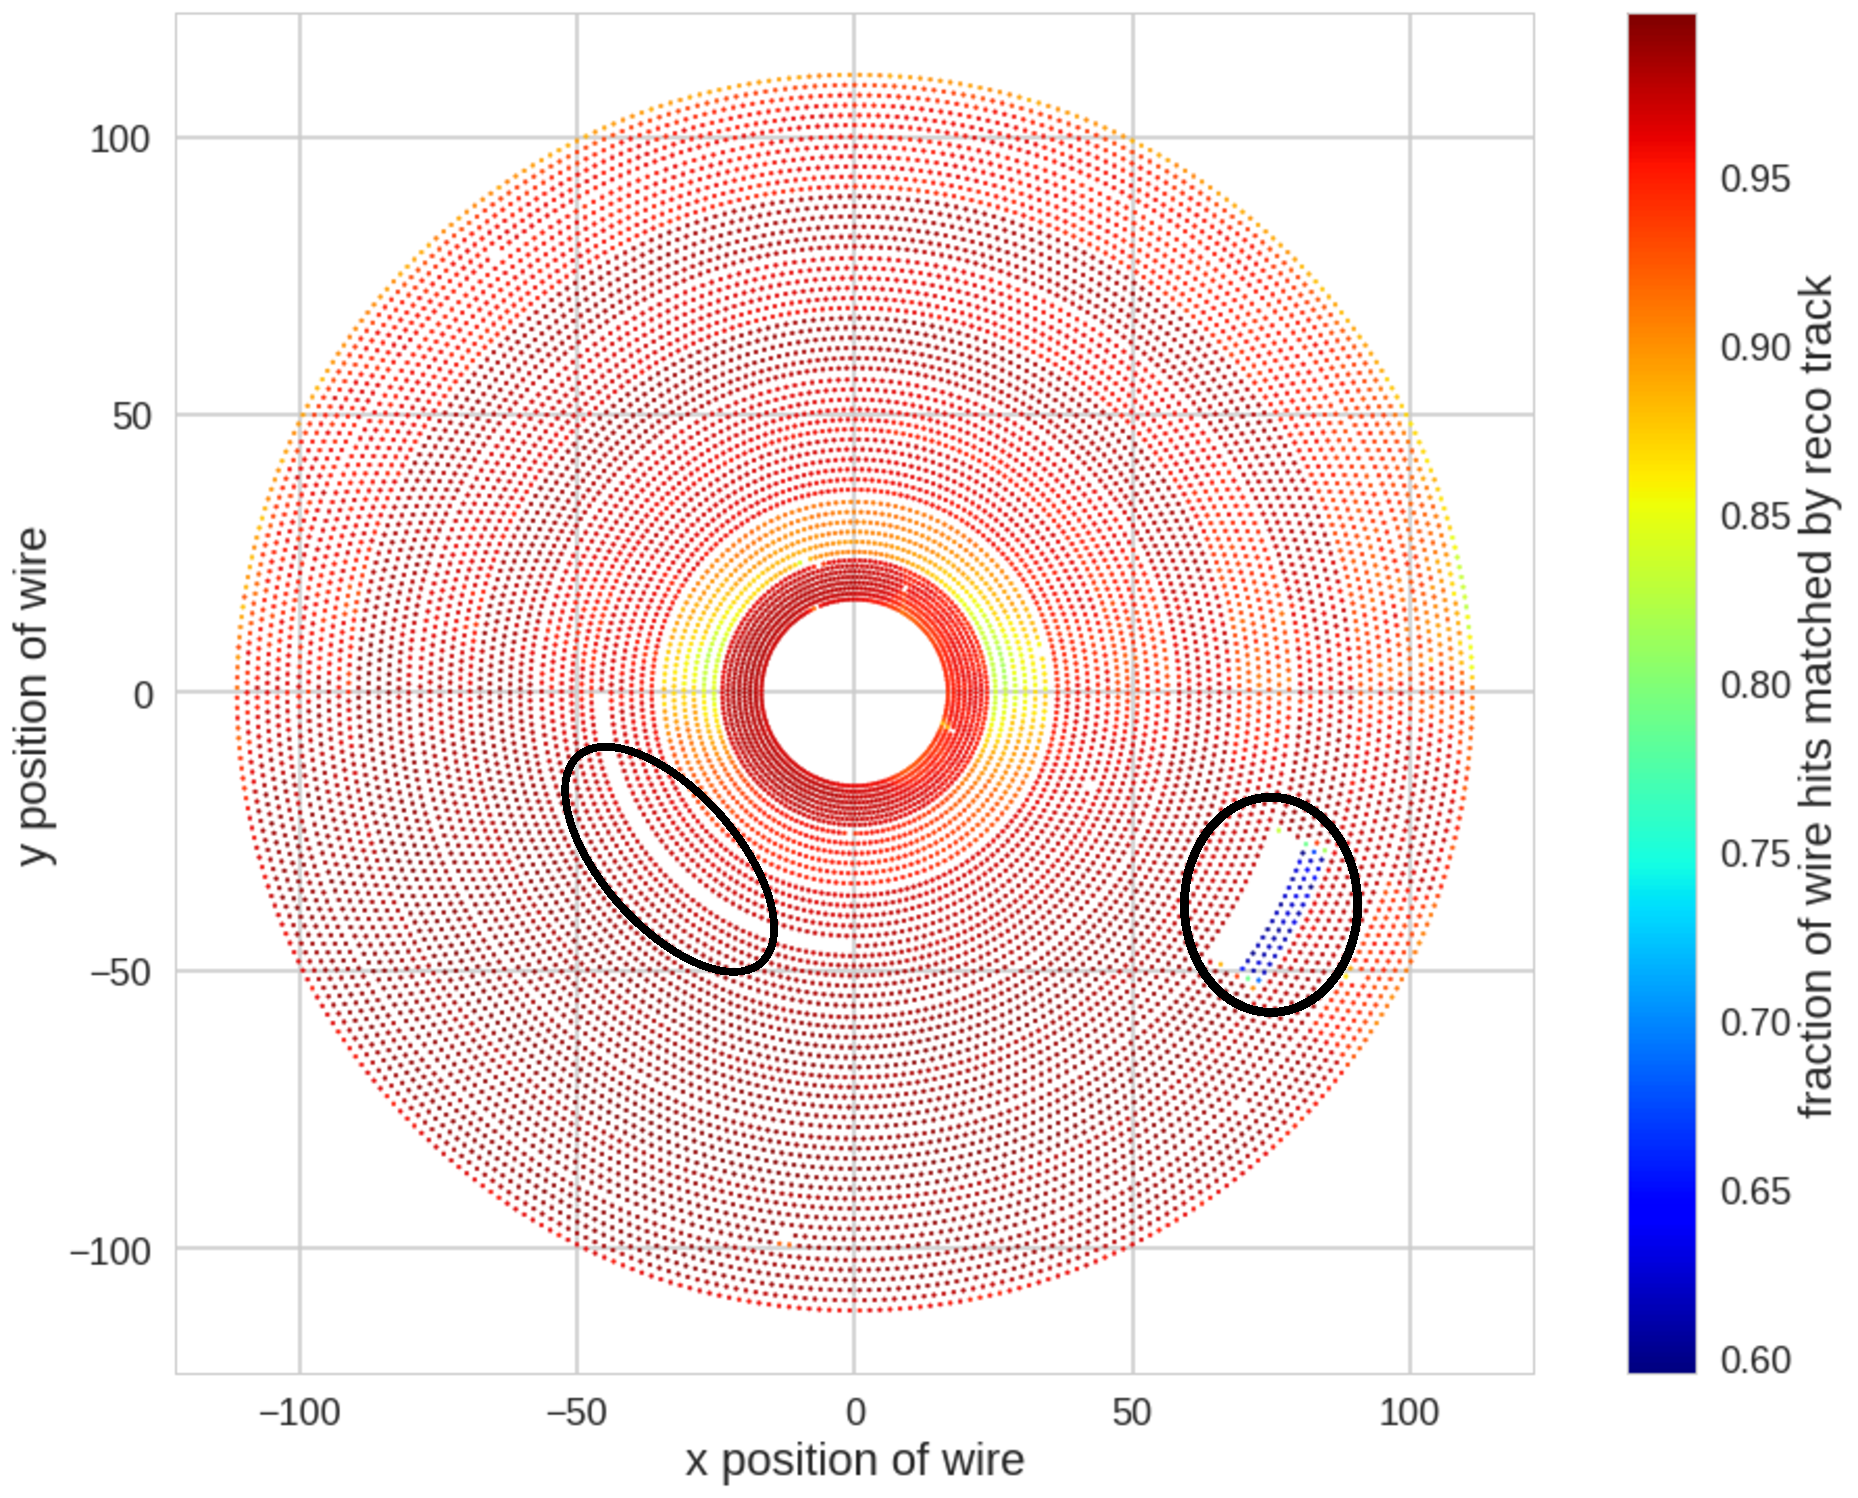
\includegraphics[width=1.\textwidth]{figures/hit_efficiency_by_wire/hit_ratio_matched_by_recotrack_MC_annotated.pdf}}
    \end{column}
  \end{columns}
  \begin{itemize}
  \item mostly flat, which is expected
  \item regions with dead channels already in simulation
  \end{itemize}
\end{frame}

\begin{frame}
  \frametitle{On GCR August measured data}
  \begin{columns}
    \begin{column}{0.5\textwidth}
      \centering
      Total hits per wire
      \includegraphics[width=1.\textwidth]{figures/hit_efficiency_by_wire/total_hits_per_wire.pdf}
    \end{column}
    \begin{column}{0.5\textwidth}
      \centering
      Fraction of hits in a reco track
      \only<1>{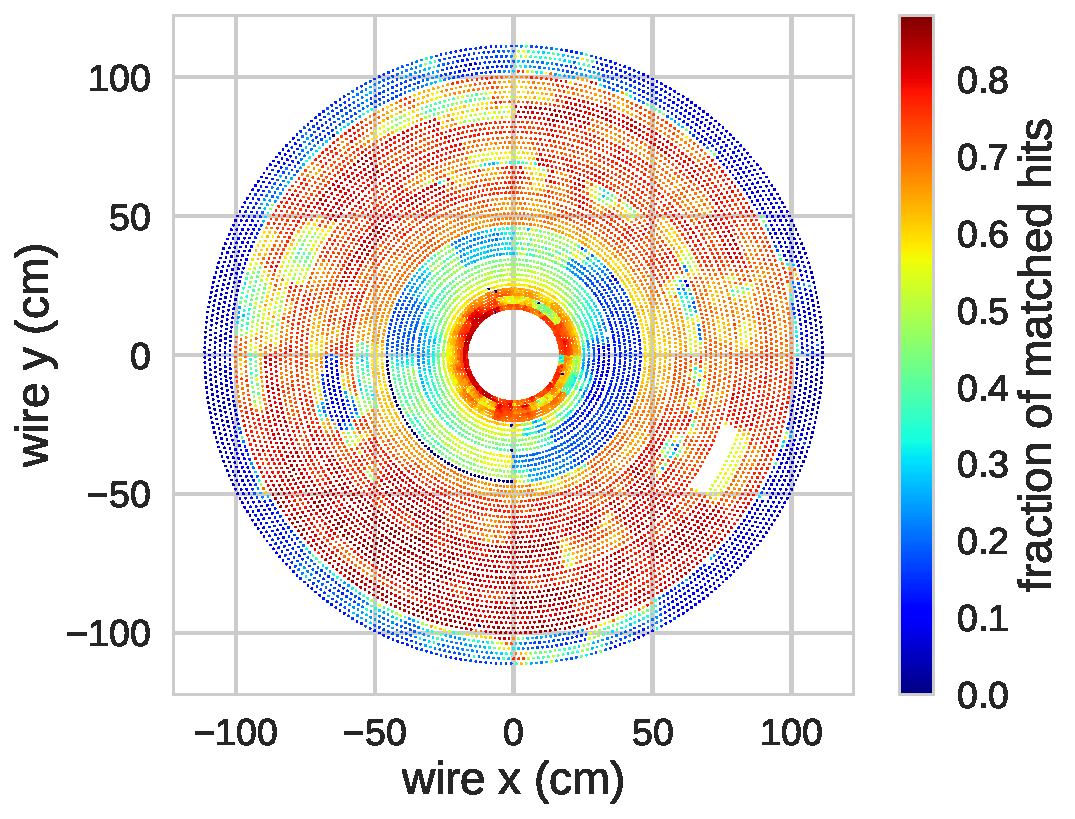
\includegraphics[width=1.\textwidth]{figures/hit_efficiency_by_wire/hit_ratio_matched_by_recotrack.pdf}}
      \only<2>{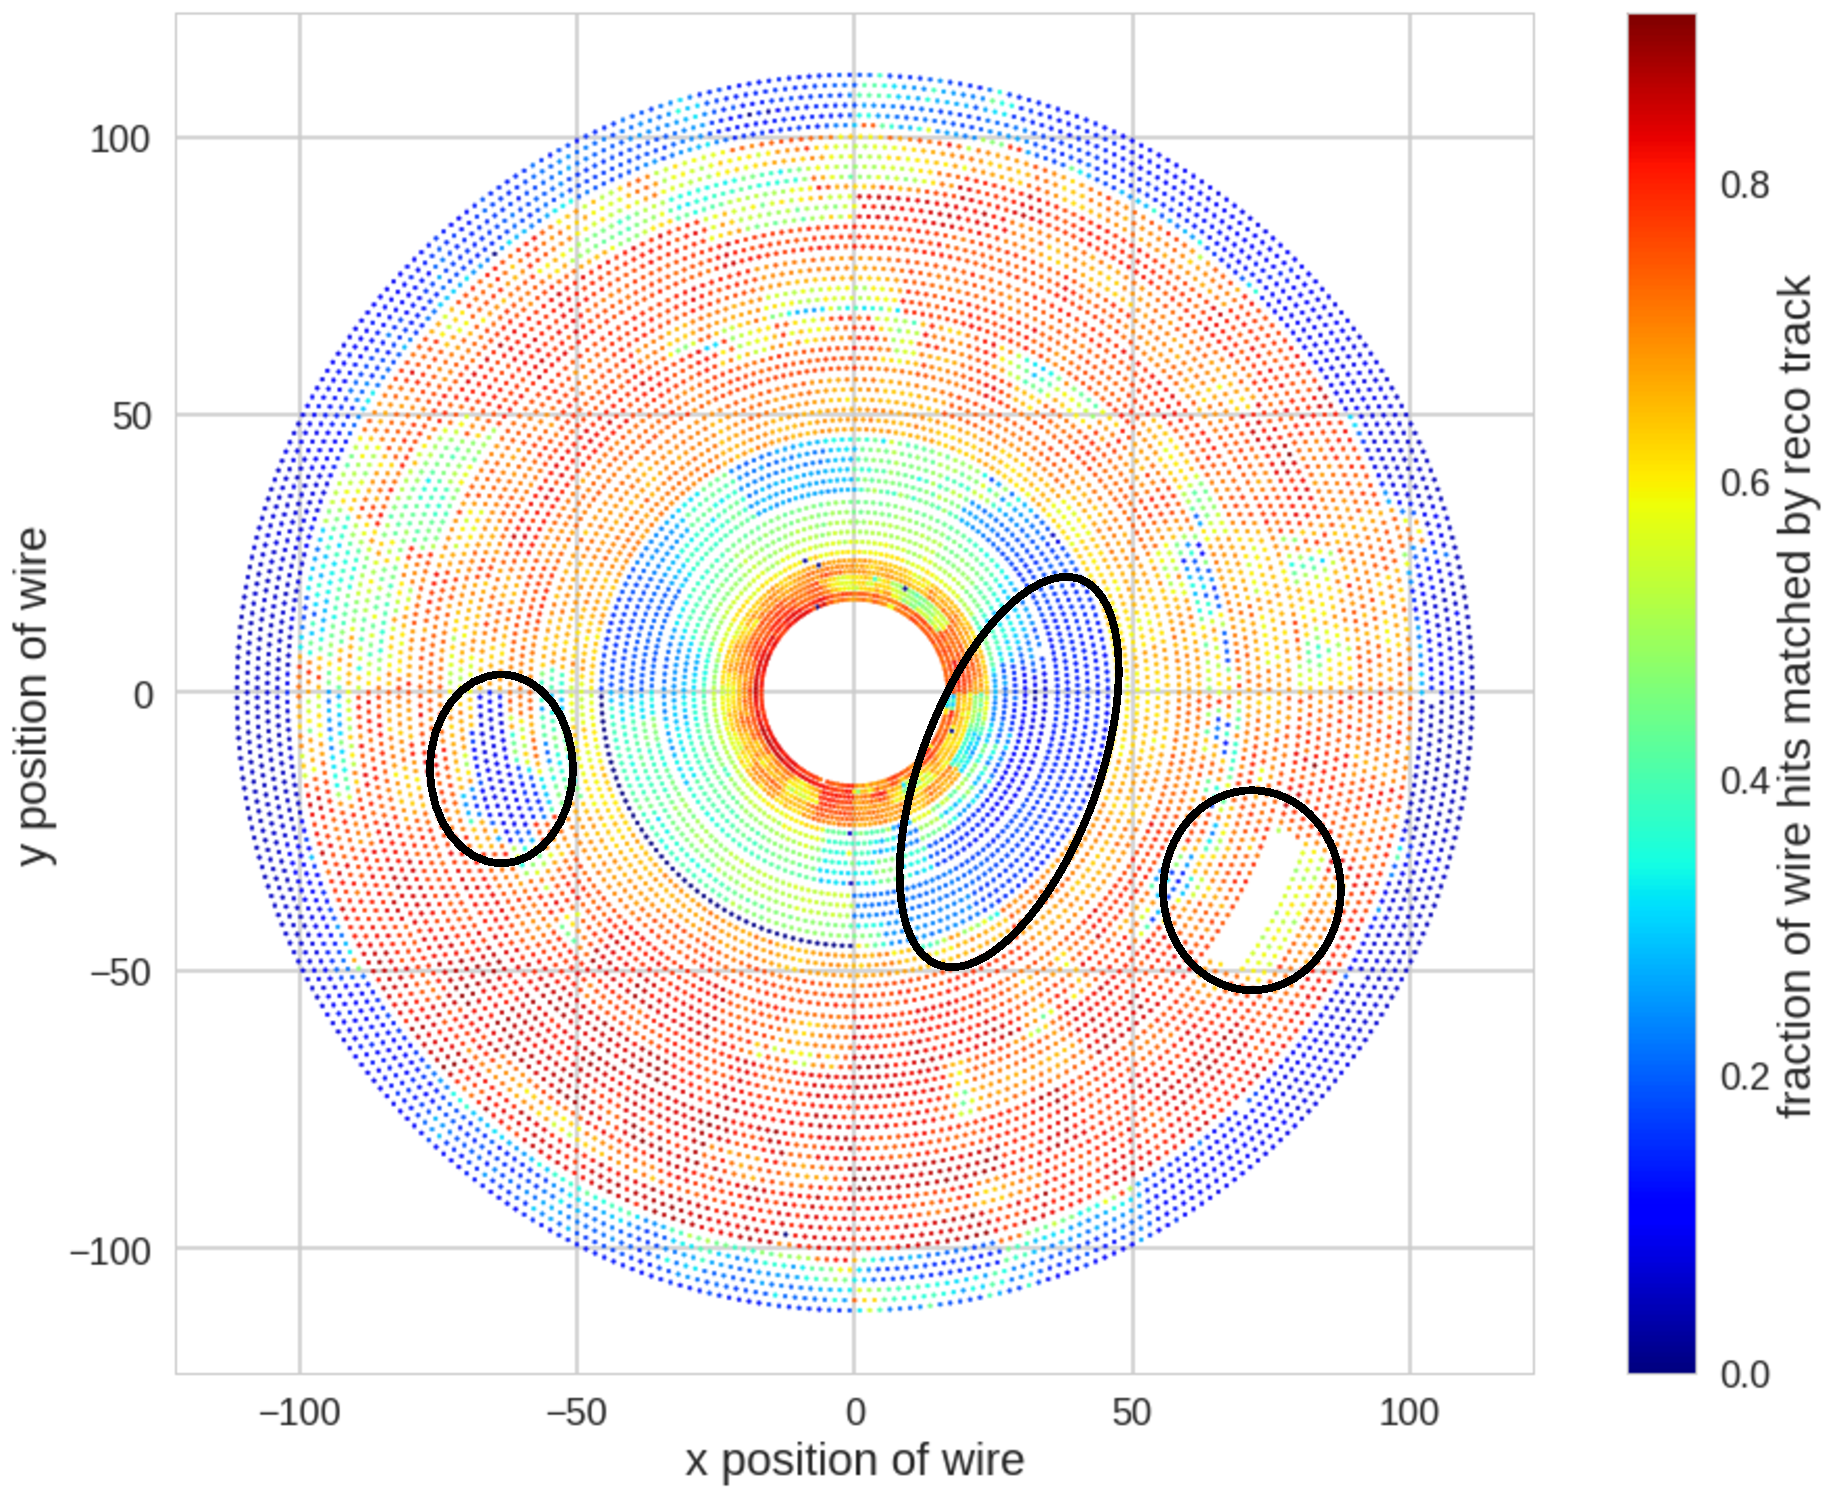
\includegraphics[width=1.\textwidth]{figures/hit_efficiency_by_wire/hit_ratio_matched_by_recotrack_annotated.pdf}}
    \end{column}
  \end{columns}
  \begin{itemize}
  \item a lot of structure visible
  \item again dead region in bottom right (superlayer 7)
  \item Superlayers 2, 3 and all of 9 (outside) noisy, a lot of unmatched hits. 
  \end{itemize}
\end{frame}

\begin{frame}
  \frametitle{Summary and Questions}\label{lastbeforebackup}
  \begin{itemize}
  \item Regions with dead wires in GCR
    \begin{itemize}
    \item Are the reasons known?
    \item Can that be fixed and are there plans?
    \end{itemize}
  \item Noisy regions:
    \begin{itemize}
    \item regions with many unmatched hits, e.g. superlayers 2, 3 and 9
    \item Is that known? Are there ideas, what the reasons might be? Noisy readout? Background?
    \end{itemize}
  \end{itemize}
\end{frame}

% \begin{frame}
%   \begin{center}
%     \huge Backup
%   \end{center}
% \end{frame}

% \begin{frame}
%   \frametitle{Hit Efficiencies by Layer}

% \end{frame}

\end{document}

%%% Local Variables:
%%% mode: latex
%%% TeX-master: t
%%% End:
